\label{section:camera_calibration}

As described in Section \ref{subsection:setup_and_tools}, a standard Gazebo ROS camera sensor is ``mounted'' to the Iris' gimbal and provides a simulated camera image as a ROS topic. The important aspects of this code are the specifications for the camera's distortion coefficients, which are all set to 0.0. Any library using a camera for image processing will require these values. Instead of passing these values to the WhyCon and April Tag libraries directly, the \texttt{calibrate\_camera} ROS module was used to generate a \texttt{.yaml} file containing the empirically determined values. This method is a de facto standard way of calibrating a camera in ROS, and can be used during migration to a physical system.
% \begin{lstlisting}[style=XML,caption={Instantiation of a Gazebo ROS camera sensor.},captionpos=b,label={lst:camera_sensor_instantiation}]
% <plugin name="camera_controller" filename="libgazebo_ros_camera.so">
%     <alwaysOn>true</alwaysOn>
%     <updateRate>0.0</updateRate>
%     <robotNamespace>/</robotNamespace>
%     <cameraName>camera</cameraName>
%     <imageTopicName>image_raw</imageTopicName>
%     <cameraInfoTopicName>camera_info</cameraInfoTopicName>
%     <frameName>camera_link</frameName>
%     <distortionK1>0.0</distortionK1>
%     <distortionK2>0.0</distortionK2>
%     <distortionK3>0.0</distortionK3>
%     <distortionT1>0.0</distortionT1>
%     <distortionT2>0.0</distortionT2>
% </plugin>
% \end{lstlisting}
%<hackBaseline>0.07</hackBaseline>
The \texttt{calibrate\_camera} script requires a rectangular ``chessboard'' defined by $m-1$ and $n-1$ where $m$ is the amount of squares along one side, and $n$ is the amount of squares along a perpendicular side. This chessboard was inserted into \texttt{sandbox.world} as a texture, as shown in Figure \ref{fig:camera_calibration}. The sizes of the squares in the chessboard are an important factor in calibration, and they were approximately the size of a single 1-meter grid square. The drone was directed around the chessboard in order to view it from many angles and distances, after which a calibration file was generated.

\begin{figure}[ht]
    \begin{subfigure}[b]{0.48\textwidth}
        \centering
        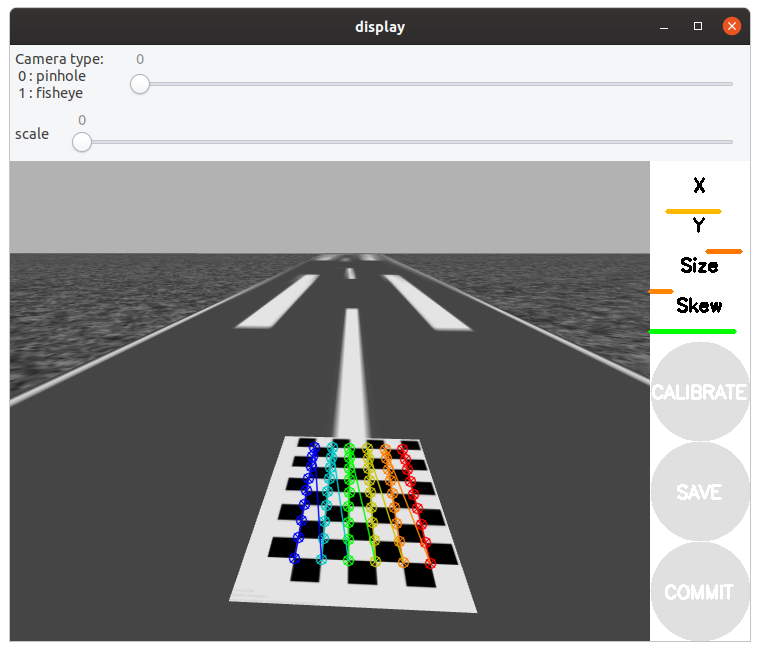
\includegraphics[height=5cm]{images/calibration_camera_view.png}
        \caption{``Chessboard'' detection.}
        \label{subfig:calibration_camera_view}
    \end{subfigure}
    \begin{subfigure}[b]{0.48\textwidth}
        \centering
        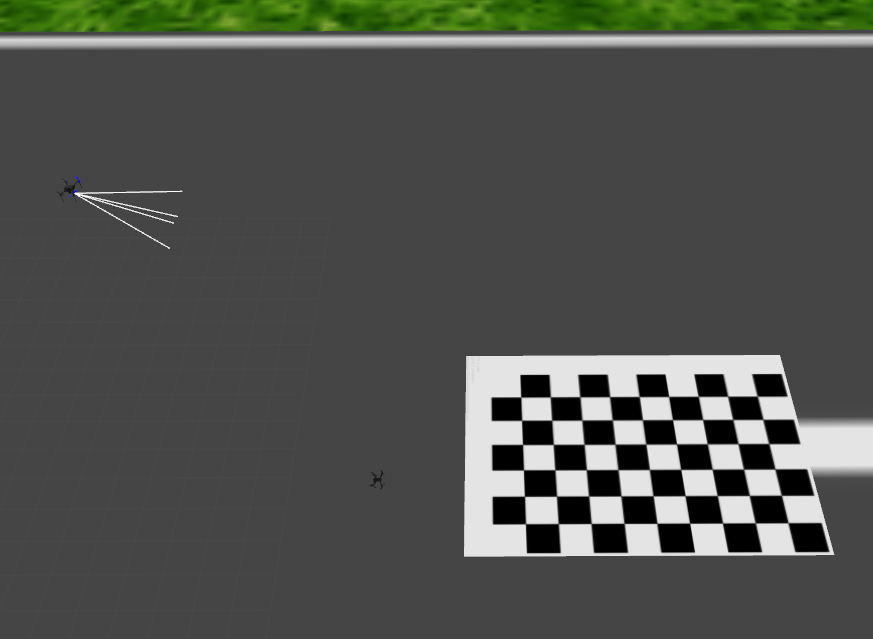
\includegraphics[height=5cm]{images/calibration_birds_eye_view.png}
        \caption{The calibration ``chessboard'' from above.}
        \label{subfig:calibration_birds_eye_view}
    \end{subfigure}
    \caption{Calibration of the simulated camera.}
    \label{fig:camera_calibration}
\end{figure}

The calibration generated the following data which has been rounded for conciseness. The camera intrinsics matrix $K$ contains $f_x, f_y$ which are the focal lengths of the camera in the $x$ and $y$ dimensions respectively, in pixel units. It also contains $c_x, c_y$ which represent the coordinates of a principal point that should be near the image center. After calibration, the simulated camera sensor is calculated to have focal lengths $f_x, f_y$ of 398.2 and 390.8 pixels respectively. With a resolution of 640x480 pixels, the calibrated values of $c_x=299.9$ and $c_y=227.5$ are only \textit{near} the image center - slightly to the upper left.

\begin{equation}
    K=
    \begin{pmatrix}
        f_x & 0 & c_x\\
        0 & f_y & c_y\\
        0 & 0 & 1
    \end{pmatrix}
    =
    \begin{pmatrix}
        398.2 & 0 & 299.9\\
        0 & 390.8 & 227.5\\
        0 & 0 & 1
    \end{pmatrix}
    \label{equation:camera_intrinsic_matrix}
\end{equation}

The distortion coefficients determined by the camera calibration, $D_T$, are roughly equivalent to those set in the camera plugin's parameters. The radial distortion coefficients $k_1, k_2, k_3$ are set to exactly zero but are calculated as only near-zero after the calibration. The tangential distortion coefficients $p_1, p_2$, corresponding to T1 and T2 in the camera plugin parameters, are also non-zero but near-zero.

\begin{equation}
    D^T=
    \begin{pmatrix}
        k_1\\k_2\\p_1\\p_2\\k_3
    \end{pmatrix}
    =
    \begin{pmatrix}
        0.0576\\-0.0321\\0.0041\\-0.0203\\0
    \end{pmatrix}
    \label{equation:distortion_coefficients}
\end{equation}

It is important to note that the process of calibrating the camera module has been developed out of necessity because typical real world cameras have non-negligible distortion coefficients. The values determined for $D^T$ are significantly lower in magnitude than those of a typical, real camera. 

% The rotation matrix $R$ determines the rotation between the first and second cameras in a stereo-vision setup. In this monocular case, the rotation is 

% \begin{equation}
%     R=
%     \begin{pmatrix}
%         1 & 0 & 0\\
%         0 & 1 & 0\\
%         0 & 0 & 1
%     \end{pmatrix}
%     \label{equation:rectification_matrix}
% \end{equation}

% \begin{equation}
%     P=
%     \begin{pmatrix}
%         406.9 & 0 & 282.8 & 0\\
%         0 & 412.1 & 229.92 & 0\\
%         0 & 0 & 1 & 0
%     \end{pmatrix}
%     \label{equation:projection_matrix}
% \end{equation}